\documentclass[twoside]{book}

% Packages required by doxygen
\usepackage{fixltx2e}
\usepackage{calc}
\usepackage{doxygen}
\usepackage[export]{adjustbox} % also loads graphicx
\usepackage{graphicx}
\usepackage[utf8]{inputenc}
\usepackage{makeidx}
\usepackage{multicol}
\usepackage{multirow}
\PassOptionsToPackage{warn}{textcomp}
\usepackage{textcomp}
\usepackage[nointegrals]{wasysym}
\usepackage[table]{xcolor}

% Font selection
\usepackage[T1]{fontenc}
\usepackage[scaled=.90]{helvet}
\usepackage{courier}
\usepackage{amssymb}
\usepackage{sectsty}
\renewcommand{\familydefault}{\sfdefault}
\allsectionsfont{%
  \fontseries{bc}\selectfont%
  \color{darkgray}%
}
\renewcommand{\DoxyLabelFont}{%
  \fontseries{bc}\selectfont%
  \color{darkgray}%
}
\newcommand{\+}{\discretionary{\mbox{\scriptsize$\hookleftarrow$}}{}{}}

% Page & text layout
\usepackage{geometry}
\geometry{%
  a4paper,%
  top=2.5cm,%
  bottom=2.5cm,%
  left=2.5cm,%
  right=2.5cm%
}
\tolerance=750
\hfuzz=15pt
\hbadness=750
\setlength{\emergencystretch}{15pt}
\setlength{\parindent}{0cm}
\setlength{\parskip}{3ex plus 2ex minus 2ex}
\makeatletter
\renewcommand{\paragraph}{%
  \@startsection{paragraph}{4}{0ex}{-1.0ex}{1.0ex}{%
    \normalfont\normalsize\bfseries\SS@parafont%
  }%
}
\renewcommand{\subparagraph}{%
  \@startsection{subparagraph}{5}{0ex}{-1.0ex}{1.0ex}{%
    \normalfont\normalsize\bfseries\SS@subparafont%
  }%
}
\makeatother

% Headers & footers
\usepackage{fancyhdr}
\pagestyle{fancyplain}
\fancyhead[LE]{\fancyplain{}{\bfseries\thepage}}
\fancyhead[CE]{\fancyplain{}{}}
\fancyhead[RE]{\fancyplain{}{\bfseries\leftmark}}
\fancyhead[LO]{\fancyplain{}{\bfseries\rightmark}}
\fancyhead[CO]{\fancyplain{}{}}
\fancyhead[RO]{\fancyplain{}{\bfseries\thepage}}
\fancyfoot[LE]{\fancyplain{}{}}
\fancyfoot[CE]{\fancyplain{}{}}
\fancyfoot[RE]{\fancyplain{}{\bfseries\scriptsize Generated by Doxygen }}
\fancyfoot[LO]{\fancyplain{}{\bfseries\scriptsize Generated by Doxygen }}
\fancyfoot[CO]{\fancyplain{}{}}
\fancyfoot[RO]{\fancyplain{}{}}
\renewcommand{\footrulewidth}{0.4pt}
\renewcommand{\chaptermark}[1]{%
  \markboth{#1}{}%
}
\renewcommand{\sectionmark}[1]{%
  \markright{\thesection\ #1}%
}

% Indices & bibliography
\usepackage{natbib}
\usepackage[titles]{tocloft}
\setcounter{tocdepth}{3}
\setcounter{secnumdepth}{5}
\makeindex

% Hyperlinks (required, but should be loaded last)
\usepackage{ifpdf}
\ifpdf
  \usepackage[pdftex,pagebackref=true]{hyperref}
\else
  \usepackage[ps2pdf,pagebackref=true]{hyperref}
\fi
\hypersetup{%
  colorlinks=true,%
  linkcolor=blue,%
  citecolor=blue,%
  unicode%
}

% Custom commands
\newcommand{\clearemptydoublepage}{%
  \newpage{\pagestyle{empty}\cleardoublepage}%
}

\usepackage{caption}
\captionsetup{labelsep=space,justification=centering,font={bf},singlelinecheck=off,skip=4pt,position=top}

%===== C O N T E N T S =====

\begin{document}

% Titlepage & ToC
\hypersetup{pageanchor=false,
             bookmarksnumbered=true,
             pdfencoding=unicode
            }
\pagenumbering{roman}
\begin{titlepage}
\vspace*{7cm}
\begin{center}%
{\Large My Project }\\
\vspace*{1cm}
{\large Generated by Doxygen 1.8.11}\\
\end{center}
\end{titlepage}
\clearemptydoublepage
\tableofcontents
\clearemptydoublepage
\pagenumbering{arabic}
\hypersetup{pageanchor=true}

%--- Begin generated contents ---
\chapter{Hierarchical Index}
\section{Class Hierarchy}
This inheritance list is sorted roughly, but not completely, alphabetically\+:\begin{DoxyCompactList}
\item \contentsline{section}{Ambi\+Connector}{\pageref{classAmbiConnector}}{}
\item \contentsline{section}{Border\+Provider}{\pageref{classBorderProvider}}{}
\begin{DoxyCompactList}
\item \contentsline{section}{Triple\+Screen\+Border\+Provider}{\pageref{classTripleScreenBorderProvider}}{}
\end{DoxyCompactList}
\item \contentsline{section}{Rgb\+Converter}{\pageref{classRgbConverter}}{}
\item runtime\+\_\+error\begin{DoxyCompactList}
\item \contentsline{section}{Ambi\+Connector\+Exception}{\pageref{classAmbiConnectorException}}{}
\begin{DoxyCompactList}
\item \contentsline{section}{Ambi\+Connector\+Communication\+Exception}{\pageref{classAmbiConnectorCommunicationException}}{}
\item \contentsline{section}{Ambi\+Connector\+Protocol\+Exception}{\pageref{classAmbiConnectorProtocolException}}{}
\end{DoxyCompactList}
\end{DoxyCompactList}
\item \contentsline{section}{Screenshot}{\pageref{classScreenshot}}{}
\begin{DoxyCompactList}
\item \contentsline{section}{Vlc\+Screenshot}{\pageref{classVlcScreenshot}}{}
\item \contentsline{section}{Xlib\+Screenshot}{\pageref{classXlibScreenshot}}{}
\end{DoxyCompactList}
\end{DoxyCompactList}

\chapter{Class Index}
\section{Class List}
Here are the classes, structs, unions and interfaces with brief descriptions\+:\begin{DoxyCompactList}
\item\contentsline{section}{\hyperlink{classAmbiConnector}{Ambi\+Connector} \\*The \hyperlink{classAmbiConnector}{Ambi\+Connector} retrieves the image data from a \hyperlink{classBorderProvider}{Border\+Provider} and sends it to an Arduino }{\pageref{classAmbiConnector}}{}
\item\contentsline{section}{\hyperlink{classAmbiConnectorCommunicationException}{Ambi\+Connector\+Communication\+Exception} \\*Exception for serial communication errors }{\pageref{classAmbiConnectorCommunicationException}}{}
\item\contentsline{section}{\hyperlink{classAmbiConnectorException}{Ambi\+Connector\+Exception} \\*Exceptions occuring in the \hyperlink{classAmbiConnector}{Ambi\+Connector} }{\pageref{classAmbiConnectorException}}{}
\item\contentsline{section}{\hyperlink{classAmbiConnectorProtocolException}{Ambi\+Connector\+Protocol\+Exception} \\*Exception for protocol errors (eg arduino not behaving as expected) }{\pageref{classAmbiConnectorProtocolException}}{}
\item\contentsline{section}{\hyperlink{classBorderProvider}{Border\+Provider} \\*Implementations encapsulate all screen information, providing only border images }{\pageref{classBorderProvider}}{}
\item\contentsline{section}{\hyperlink{classRgbConverter}{Rgb\+Converter} \\*Link between the \hyperlink{classBorderProvider}{Border\+Provider} images and raw R\+GB data for the arduino }{\pageref{classRgbConverter}}{}
\item\contentsline{section}{\hyperlink{classScreenshot}{Screenshot} \\*Interface for capturing screen areas }{\pageref{classScreenshot}}{}
\item\contentsline{section}{\hyperlink{classTripleScreenBorderProvider}{Triple\+Screen\+Border\+Provider} \\*An implementation of \hyperlink{classBorderProvider}{Border\+Provider}, accessing three monitors via the Screen\+Shot class }{\pageref{classTripleScreenBorderProvider}}{}
\item\contentsline{section}{\hyperlink{classVlcScreenshot}{Vlc\+Screenshot} \\*An implementation of the \hyperlink{classScreenshot}{Screenshot} interface; it reads from a video stream provided by vlc. Not finished! }{\pageref{classVlcScreenshot}}{}
\item\contentsline{section}{\hyperlink{classXlibScreenshot}{Xlib\+Screenshot} \\*An implementation of the \hyperlink{classScreenshot}{Screenshot} interface; uses xlib }{\pageref{classXlibScreenshot}}{}
\end{DoxyCompactList}

\chapter{Class Documentation}
\hypertarget{classAmbiConnector}{}\section{Ambi\+Connector Class Reference}
\label{classAmbiConnector}\index{Ambi\+Connector@{Ambi\+Connector}}


The \hyperlink{classAmbiConnector}{Ambi\+Connector} retrieves the image data from a \hyperlink{classBorderProvider}{Border\+Provider} and sends it to an Arduino.  




{\ttfamily \#include $<$ambiconnector.\+h$>$}

\subsection*{Public Member Functions}
\begin{DoxyCompactItemize}
\item 
void \hyperlink{classAmbiConnector_af12c0b2034feb3016279672449009ae2}{update} ()\hypertarget{classAmbiConnector_af12c0b2034feb3016279672449009ae2}{}\label{classAmbiConnector_af12c0b2034feb3016279672449009ae2}

\begin{DoxyCompactList}\small\item\em update screen data \end{DoxyCompactList}\item 
void \hyperlink{classAmbiConnector_a9298de50c73e9dfd204baccc4fc1afab}{draw} ()\hypertarget{classAmbiConnector_a9298de50c73e9dfd204baccc4fc1afab}{}\label{classAmbiConnector_a9298de50c73e9dfd204baccc4fc1afab}

\begin{DoxyCompactList}\small\item\em push current data to leds \end{DoxyCompactList}\item 
bool \hyperlink{classAmbiConnector_ab093d68899b581349a0e2479c25da2ca}{connect} (const std\+::\+\_\+\+\_\+cxx11\+::string \&port)
\begin{DoxyCompactList}\small\item\em connect to the arduino; because it waits for established comms, it is blocking \end{DoxyCompactList}\item 
float \hyperlink{classAmbiConnector_acfd5219af9b1c1d7d7dfdfac420c970a}{get\+Current\+Fps} ()
\begin{DoxyCompactList}\small\item\em calculate and return the current fps, measured by completed draw calls \end{DoxyCompactList}\item 
\hyperlink{classAmbiConnector_a72b592fc07d3b3ea297d00cb9b87b1bc}{Ambi\+Connector} (std\+::shared\+\_\+ptr$<$ \hyperlink{classBorderProvider}{Border\+Provider} $>$ border\+Provider, unsigned int horizontal\+Led\+Count, unsigned int vertical\+Led\+Count)
\begin{DoxyCompactList}\small\item\em construct an \hyperlink{classAmbiConnector}{Ambi\+Connector}, responsible for obtaining and updating the led data \end{DoxyCompactList}\end{DoxyCompactItemize}


\subsection{Detailed Description}
The \hyperlink{classAmbiConnector}{Ambi\+Connector} retrieves the image data from a \hyperlink{classBorderProvider}{Border\+Provider} and sends it to an Arduino. 

\subsection{Constructor \& Destructor Documentation}
\index{Ambi\+Connector@{Ambi\+Connector}!Ambi\+Connector@{Ambi\+Connector}}
\index{Ambi\+Connector@{Ambi\+Connector}!Ambi\+Connector@{Ambi\+Connector}}
\subsubsection[{\texorpdfstring{Ambi\+Connector(std\+::shared\+\_\+ptr$<$ Border\+Provider $>$ border\+Provider, unsigned int horizontal\+Led\+Count, unsigned int vertical\+Led\+Count)}{AmbiConnector(std::shared_ptr< BorderProvider > borderProvider, unsigned int horizontalLedCount, unsigned int verticalLedCount)}}]{\setlength{\rightskip}{0pt plus 5cm}Ambi\+Connector\+::\+Ambi\+Connector (
\begin{DoxyParamCaption}
\item[{std\+::shared\+\_\+ptr$<$ {\bf Border\+Provider} $>$}]{border\+Provider, }
\item[{unsigned int}]{horizontal\+Led\+Count, }
\item[{unsigned int}]{vertical\+Led\+Count}
\end{DoxyParamCaption}
)}\hypertarget{classAmbiConnector_a72b592fc07d3b3ea297d00cb9b87b1bc}{}\label{classAmbiConnector_a72b592fc07d3b3ea297d00cb9b87b1bc}


construct an \hyperlink{classAmbiConnector}{Ambi\+Connector}, responsible for obtaining and updating the led data 


\begin{DoxyParams}{Parameters}
{\em border\+Provider} & will be used to obtain the border images \\
\hline
{\em horizontal\+Led\+Count} & how many leds are on each horizontal border \\
\hline
{\em vertical\+Led\+Count} & how many leds are on each vertical border \\
\hline
\end{DoxyParams}


\subsection{Member Function Documentation}
\index{Ambi\+Connector@{Ambi\+Connector}!connect@{connect}}
\index{connect@{connect}!Ambi\+Connector@{Ambi\+Connector}}
\subsubsection[{\texorpdfstring{connect(const std\+::\+\_\+\+\_\+cxx11\+::string \&port)}{connect(const std::__cxx11::string &port)}}]{\setlength{\rightskip}{0pt plus 5cm}bool Ambi\+Connector\+::connect (
\begin{DoxyParamCaption}
\item[{const std\+::\+\_\+\+\_\+cxx11\+::string \&}]{port}
\end{DoxyParamCaption}
)}\hypertarget{classAmbiConnector_ab093d68899b581349a0e2479c25da2ca}{}\label{classAmbiConnector_ab093d68899b581349a0e2479c25da2ca}


connect to the arduino; because it waits for established comms, it is blocking 

\begin{DoxyReturn}{Returns}
true if connection establishment successfull 
\end{DoxyReturn}
\index{Ambi\+Connector@{Ambi\+Connector}!get\+Current\+Fps@{get\+Current\+Fps}}
\index{get\+Current\+Fps@{get\+Current\+Fps}!Ambi\+Connector@{Ambi\+Connector}}
\subsubsection[{\texorpdfstring{get\+Current\+Fps()}{getCurrentFps()}}]{\setlength{\rightskip}{0pt plus 5cm}float Ambi\+Connector\+::get\+Current\+Fps (
\begin{DoxyParamCaption}
{}
\end{DoxyParamCaption}
)\hspace{0.3cm}{\ttfamily [inline]}}\hypertarget{classAmbiConnector_acfd5219af9b1c1d7d7dfdfac420c970a}{}\label{classAmbiConnector_acfd5219af9b1c1d7d7dfdfac420c970a}


calculate and return the current fps, measured by completed draw calls 

\begin{DoxyReturn}{Returns}
current fps 
\end{DoxyReturn}


The documentation for this class was generated from the following files\+:\begin{DoxyCompactItemize}
\item 
ambiconnector.\+h\item 
ambiconnector.\+cpp\end{DoxyCompactItemize}

\hypertarget{classAmbiConnectorCommunicationException}{}\section{Ambi\+Connector\+Communication\+Exception Class Reference}
\label{classAmbiConnectorCommunicationException}\index{Ambi\+Connector\+Communication\+Exception@{Ambi\+Connector\+Communication\+Exception}}


Exception for serial communication errors.  




{\ttfamily \#include $<$ledexceptions.\+h$>$}

Inheritance diagram for Ambi\+Connector\+Communication\+Exception\+:\begin{figure}[H]
\begin{center}
\leavevmode
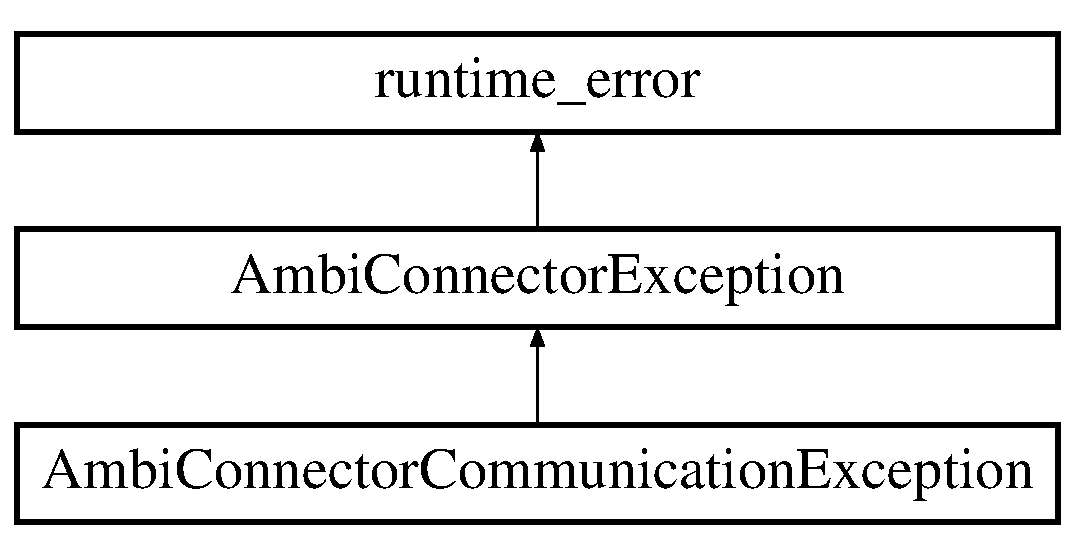
\includegraphics[height=3.000000cm]{classAmbiConnectorCommunicationException}
\end{center}
\end{figure}
\subsection*{Public Member Functions}
\begin{DoxyCompactItemize}
\item 
\hyperlink{classAmbiConnectorCommunicationException_a41f8ac30337b6f1e0c6f3562d42fbbb3}{Ambi\+Connector\+Communication\+Exception} (const std\+::string \&message)
\begin{DoxyCompactList}\small\item\em std\+::string constructor \end{DoxyCompactList}\end{DoxyCompactItemize}


\subsection{Detailed Description}
Exception for serial communication errors. 

\subsection{Constructor \& Destructor Documentation}
\index{Ambi\+Connector\+Communication\+Exception@{Ambi\+Connector\+Communication\+Exception}!Ambi\+Connector\+Communication\+Exception@{Ambi\+Connector\+Communication\+Exception}}
\index{Ambi\+Connector\+Communication\+Exception@{Ambi\+Connector\+Communication\+Exception}!Ambi\+Connector\+Communication\+Exception@{Ambi\+Connector\+Communication\+Exception}}
\subsubsection[{\texorpdfstring{Ambi\+Connector\+Communication\+Exception(const std\+::string \&message)}{AmbiConnectorCommunicationException(const std::string &message)}}]{\setlength{\rightskip}{0pt plus 5cm}Ambi\+Connector\+Communication\+Exception\+::\+Ambi\+Connector\+Communication\+Exception (
\begin{DoxyParamCaption}
\item[{const std\+::string \&}]{message}
\end{DoxyParamCaption}
)\hspace{0.3cm}{\ttfamily [inline]}}\hypertarget{classAmbiConnectorCommunicationException_a41f8ac30337b6f1e0c6f3562d42fbbb3}{}\label{classAmbiConnectorCommunicationException_a41f8ac30337b6f1e0c6f3562d42fbbb3}


std\+::string constructor 


\begin{DoxyParams}{Parameters}
{\em message} & the error message \\
\hline
\end{DoxyParams}


The documentation for this class was generated from the following file\+:\begin{DoxyCompactItemize}
\item 
ledexceptions.\+h\end{DoxyCompactItemize}

\hypertarget{classAmbiConnectorException}{}\section{Ambi\+Connector\+Exception Class Reference}
\label{classAmbiConnectorException}\index{Ambi\+Connector\+Exception@{Ambi\+Connector\+Exception}}


Exceptions occuring in the \hyperlink{classAmbiConnector}{Ambi\+Connector}.  




{\ttfamily \#include $<$ledexceptions.\+h$>$}

Inheritance diagram for Ambi\+Connector\+Exception\+:\begin{figure}[H]
\begin{center}
\leavevmode
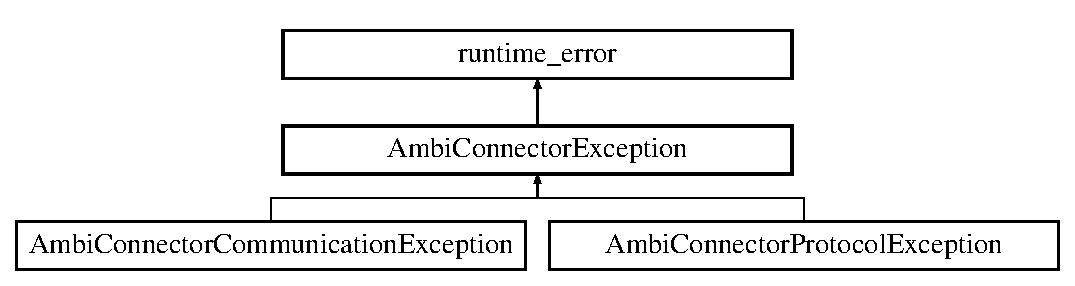
\includegraphics[height=3.000000cm]{classAmbiConnectorException}
\end{center}
\end{figure}
\subsection*{Public Member Functions}
\begin{DoxyCompactItemize}
\item 
\hyperlink{classAmbiConnectorException_a3e645fd52f6383ad3420e82d82bb1fbd}{Ambi\+Connector\+Exception} (const std\+::string \&message)
\begin{DoxyCompactList}\small\item\em std\+::string constructor \end{DoxyCompactList}\end{DoxyCompactItemize}


\subsection{Detailed Description}
Exceptions occuring in the \hyperlink{classAmbiConnector}{Ambi\+Connector}. 

\subsection{Constructor \& Destructor Documentation}
\index{Ambi\+Connector\+Exception@{Ambi\+Connector\+Exception}!Ambi\+Connector\+Exception@{Ambi\+Connector\+Exception}}
\index{Ambi\+Connector\+Exception@{Ambi\+Connector\+Exception}!Ambi\+Connector\+Exception@{Ambi\+Connector\+Exception}}
\subsubsection[{\texorpdfstring{Ambi\+Connector\+Exception(const std\+::string \&message)}{AmbiConnectorException(const std::string &message)}}]{\setlength{\rightskip}{0pt plus 5cm}Ambi\+Connector\+Exception\+::\+Ambi\+Connector\+Exception (
\begin{DoxyParamCaption}
\item[{const std\+::string \&}]{message}
\end{DoxyParamCaption}
)\hspace{0.3cm}{\ttfamily [inline]}}\hypertarget{classAmbiConnectorException_a3e645fd52f6383ad3420e82d82bb1fbd}{}\label{classAmbiConnectorException_a3e645fd52f6383ad3420e82d82bb1fbd}


std\+::string constructor 


\begin{DoxyParams}{Parameters}
{\em message} & the error message \\
\hline
\end{DoxyParams}


The documentation for this class was generated from the following file\+:\begin{DoxyCompactItemize}
\item 
ledexceptions.\+h\end{DoxyCompactItemize}

\hypertarget{classAmbiConnectorProtocolException}{}\section{Ambi\+Connector\+Protocol\+Exception Class Reference}
\label{classAmbiConnectorProtocolException}\index{Ambi\+Connector\+Protocol\+Exception@{Ambi\+Connector\+Protocol\+Exception}}


Exception for protocol errors (eg arduino not behaving as expected)  




{\ttfamily \#include $<$ledexceptions.\+h$>$}

Inheritance diagram for Ambi\+Connector\+Protocol\+Exception\+:\begin{figure}[H]
\begin{center}
\leavevmode
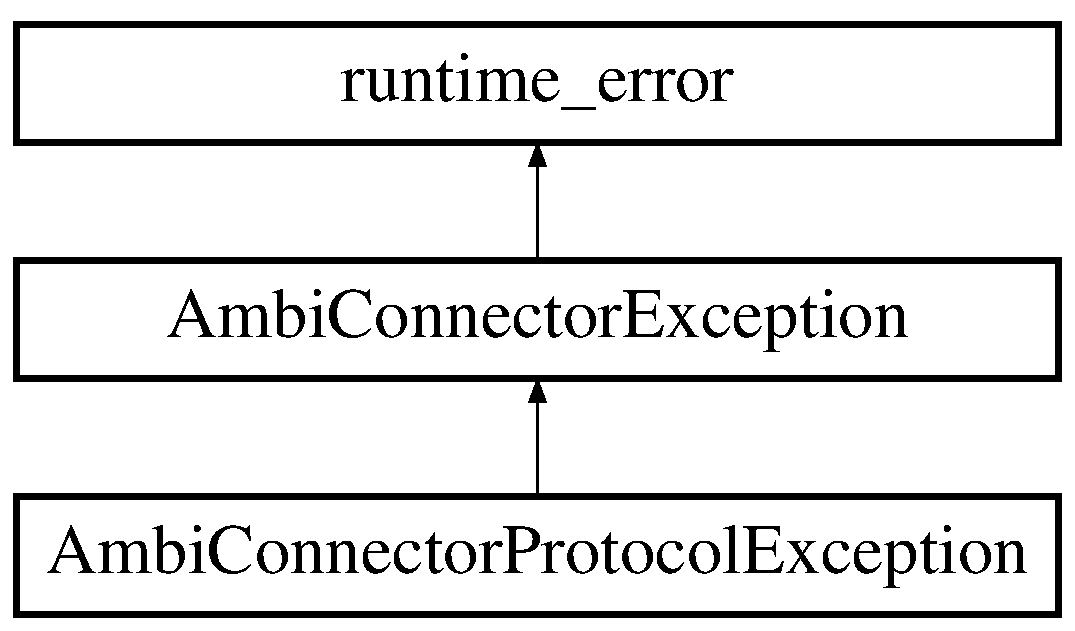
\includegraphics[height=3.000000cm]{classAmbiConnectorProtocolException}
\end{center}
\end{figure}
\subsection*{Public Member Functions}
\begin{DoxyCompactItemize}
\item 
\hyperlink{classAmbiConnectorProtocolException_a7f4fa656c11ddb28462e9441403433e7}{Ambi\+Connector\+Protocol\+Exception} (const std\+::string \&message)
\begin{DoxyCompactList}\small\item\em std\+::string constructor \end{DoxyCompactList}\end{DoxyCompactItemize}


\subsection{Detailed Description}
Exception for protocol errors (eg arduino not behaving as expected) 

\subsection{Constructor \& Destructor Documentation}
\index{Ambi\+Connector\+Protocol\+Exception@{Ambi\+Connector\+Protocol\+Exception}!Ambi\+Connector\+Protocol\+Exception@{Ambi\+Connector\+Protocol\+Exception}}
\index{Ambi\+Connector\+Protocol\+Exception@{Ambi\+Connector\+Protocol\+Exception}!Ambi\+Connector\+Protocol\+Exception@{Ambi\+Connector\+Protocol\+Exception}}
\subsubsection[{\texorpdfstring{Ambi\+Connector\+Protocol\+Exception(const std\+::string \&message)}{AmbiConnectorProtocolException(const std::string &message)}}]{\setlength{\rightskip}{0pt plus 5cm}Ambi\+Connector\+Protocol\+Exception\+::\+Ambi\+Connector\+Protocol\+Exception (
\begin{DoxyParamCaption}
\item[{const std\+::string \&}]{message}
\end{DoxyParamCaption}
)\hspace{0.3cm}{\ttfamily [inline]}}\hypertarget{classAmbiConnectorProtocolException_a7f4fa656c11ddb28462e9441403433e7}{}\label{classAmbiConnectorProtocolException_a7f4fa656c11ddb28462e9441403433e7}


std\+::string constructor 


\begin{DoxyParams}{Parameters}
{\em message} & the error message \\
\hline
\end{DoxyParams}


The documentation for this class was generated from the following file\+:\begin{DoxyCompactItemize}
\item 
ledexceptions.\+h\end{DoxyCompactItemize}

\hypertarget{classBorderProvider}{}\section{Border\+Provider Class Reference}
\label{classBorderProvider}\index{Border\+Provider@{Border\+Provider}}


Implementations encapsulate all screen information, providing only border images.  




{\ttfamily \#include $<$borderprovider.\+h$>$}

Inheritance diagram for Border\+Provider\+:\begin{figure}[H]
\begin{center}
\leavevmode
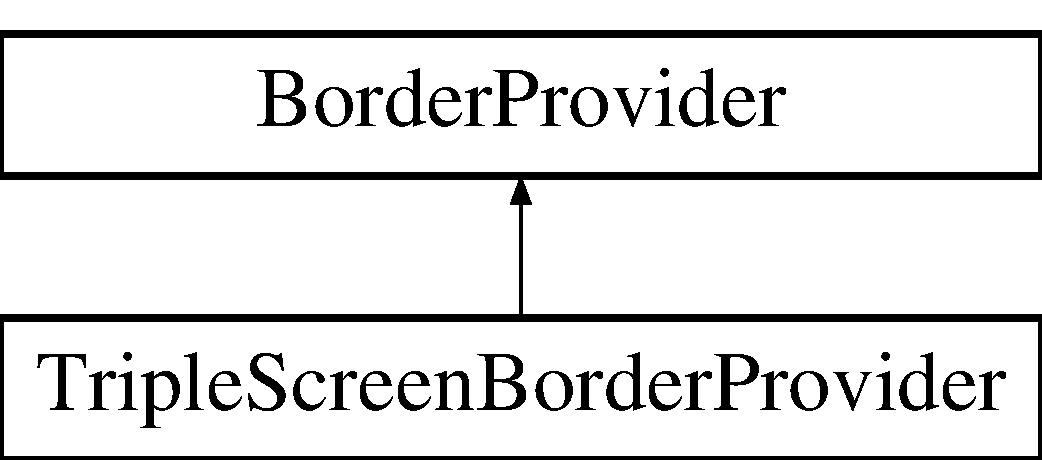
\includegraphics[height=2.000000cm]{classBorderProvider}
\end{center}
\end{figure}
\subsection*{Public Member Functions}
\begin{DoxyCompactItemize}
\item 
virtual void \hyperlink{classBorderProvider_afdad2b6203baadf45a4e7b7d243bdca9}{retrieve\+Borders} (Magick\+::\+Image \&right, Magick\+::\+Image \&top, Magick\+::\+Image \&left, Magick\+::\+Image \&bottom)=0\hypertarget{classBorderProvider_afdad2b6203baadf45a4e7b7d243bdca9}{}\label{classBorderProvider_afdad2b6203baadf45a4e7b7d243bdca9}

\begin{DoxyCompactList}\small\item\em This function must capture each screen border into a Magick++ image. \end{DoxyCompactList}\end{DoxyCompactItemize}


\subsection{Detailed Description}
Implementations encapsulate all screen information, providing only border images. 

The documentation for this class was generated from the following file\+:\begin{DoxyCompactItemize}
\item 
borderprovider.\+h\end{DoxyCompactItemize}

\hypertarget{classRgbConverter}{}\section{Rgb\+Converter Class Reference}
\label{classRgbConverter}\index{Rgb\+Converter@{Rgb\+Converter}}


The \hyperlink{classRgbConverter}{Rgb\+Converter} class is the link between the \hyperlink{classBorderProvider}{Border\+Provider} images and raw R\+GB data for the arduino.  




{\ttfamily \#include $<$rgbconstructor.\+h$>$}

\subsection*{Public Member Functions}
\begin{DoxyCompactItemize}
\item 
\hyperlink{classRgbConverter_a1a88728db70b694de8702716d3f4f0e8}{Rgb\+Converter} (std\+::shared\+\_\+ptr$<$ \hyperlink{classBorderProvider}{Border\+Provider} $>$ provider, unsigned int horizontal\+Led\+Count, unsigned int vertical\+Led\+Count)
\begin{DoxyCompactList}\small\item\em create a new rgb constructor object \end{DoxyCompactList}\item 
float \hyperlink{classRgbConverter_a37985f601284a5a90e4fee7485085da8}{take\+And\+Parse\+Screen\+Shot} (uint8\+\_\+t $\ast$result\+Space)
\begin{DoxyCompactList}\small\item\em Retrieves border images and provides rgb output data. \end{DoxyCompactList}\item 
size\+\_\+t \hyperlink{classRgbConverter_aa6ad1b8cc5f4a9fa3e7304e1884f9a8c}{get\+Required\+Buffer\+Length} () const 
\begin{DoxyCompactList}\small\item\em Access the required result buffer length. \end{DoxyCompactList}\item 
void \hyperlink{classRgbConverter_a070b03c9ecd6bf1f801403cc4ed99d50}{set\+Brightness\+Factor} (float val)
\begin{DoxyCompactList}\small\item\em Set a factor for all channel brightnesses. \end{DoxyCompactList}\end{DoxyCompactItemize}


\subsection{Detailed Description}
The \hyperlink{classRgbConverter}{Rgb\+Converter} class is the link between the \hyperlink{classBorderProvider}{Border\+Provider} images and raw R\+GB data for the arduino. 

\subsection{Constructor \& Destructor Documentation}
\index{Rgb\+Converter@{Rgb\+Converter}!Rgb\+Converter@{Rgb\+Converter}}
\index{Rgb\+Converter@{Rgb\+Converter}!Rgb\+Converter@{Rgb\+Converter}}
\subsubsection[{\texorpdfstring{Rgb\+Converter(std\+::shared\+\_\+ptr$<$ Border\+Provider $>$ provider, unsigned int horizontal\+Led\+Count, unsigned int vertical\+Led\+Count)}{RgbConverter(std::shared_ptr< BorderProvider > provider, unsigned int horizontalLedCount, unsigned int verticalLedCount)}}]{\setlength{\rightskip}{0pt plus 5cm}Rgb\+Converter\+::\+Rgb\+Converter (
\begin{DoxyParamCaption}
\item[{std\+::shared\+\_\+ptr$<$ {\bf Border\+Provider} $>$}]{provider, }
\item[{unsigned int}]{horizontal\+Led\+Count, }
\item[{unsigned int}]{vertical\+Led\+Count}
\end{DoxyParamCaption}
)}\hypertarget{classRgbConverter_a1a88728db70b694de8702716d3f4f0e8}{}\label{classRgbConverter_a1a88728db70b694de8702716d3f4f0e8}


create a new rgb constructor object 


\begin{DoxyParams}{Parameters}
{\em provider} & the \hyperlink{classBorderProvider}{Border\+Provider} that will be used to capture the screen borders \\
\hline
{\em vertical\+Led\+Count} & how many leds are on each vertical border \\
\hline
{\em horizontal\+Led\+Count} & how many leds are on each horizontal border \\
\hline
\end{DoxyParams}


\subsection{Member Function Documentation}
\index{Rgb\+Converter@{Rgb\+Converter}!get\+Required\+Buffer\+Length@{get\+Required\+Buffer\+Length}}
\index{get\+Required\+Buffer\+Length@{get\+Required\+Buffer\+Length}!Rgb\+Converter@{Rgb\+Converter}}
\subsubsection[{\texorpdfstring{get\+Required\+Buffer\+Length() const }{getRequiredBufferLength() const }}]{\setlength{\rightskip}{0pt plus 5cm}size\+\_\+t Rgb\+Converter\+::get\+Required\+Buffer\+Length (
\begin{DoxyParamCaption}
{}
\end{DoxyParamCaption}
) const\hspace{0.3cm}{\ttfamily [inline]}}\hypertarget{classRgbConverter_aa6ad1b8cc5f4a9fa3e7304e1884f9a8c}{}\label{classRgbConverter_aa6ad1b8cc5f4a9fa3e7304e1884f9a8c}


Access the required result buffer length. 

\begin{DoxyReturn}{Returns}
the number of bytes required to buffer the resulting led data 
\end{DoxyReturn}
\index{Rgb\+Converter@{Rgb\+Converter}!set\+Brightness\+Factor@{set\+Brightness\+Factor}}
\index{set\+Brightness\+Factor@{set\+Brightness\+Factor}!Rgb\+Converter@{Rgb\+Converter}}
\subsubsection[{\texorpdfstring{set\+Brightness\+Factor(float val)}{setBrightnessFactor(float val)}}]{\setlength{\rightskip}{0pt plus 5cm}void Rgb\+Converter\+::set\+Brightness\+Factor (
\begin{DoxyParamCaption}
\item[{float}]{val}
\end{DoxyParamCaption}
)\hspace{0.3cm}{\ttfamily [inline]}}\hypertarget{classRgbConverter_a070b03c9ecd6bf1f801403cc4ed99d50}{}\label{classRgbConverter_a070b03c9ecd6bf1f801403cc4ed99d50}


Set a factor for all channel brightnesses. 


\begin{DoxyParams}{Parameters}
{\em val} & new factor; values greater than 1 will be interesting... \\
\hline
\end{DoxyParams}
\index{Rgb\+Converter@{Rgb\+Converter}!take\+And\+Parse\+Screen\+Shot@{take\+And\+Parse\+Screen\+Shot}}
\index{take\+And\+Parse\+Screen\+Shot@{take\+And\+Parse\+Screen\+Shot}!Rgb\+Converter@{Rgb\+Converter}}
\subsubsection[{\texorpdfstring{take\+And\+Parse\+Screen\+Shot(uint8\+\_\+t $\ast$result\+Space)}{takeAndParseScreenShot(uint8_t *resultSpace)}}]{\setlength{\rightskip}{0pt plus 5cm}float Rgb\+Converter\+::take\+And\+Parse\+Screen\+Shot (
\begin{DoxyParamCaption}
\item[{uint8\+\_\+t $\ast$}]{result\+Space}
\end{DoxyParamCaption}
)}\hypertarget{classRgbConverter_a37985f601284a5a90e4fee7485085da8}{}\label{classRgbConverter_a37985f601284a5a90e4fee7485085da8}


Retrieves border images and provides rgb output data. 


\begin{DoxyParams}[1]{Parameters}
\mbox{\tt out}  & {\em result\+Space} & Storage provided for the rgb output data; length must be at least the value of \char`\"{}\+::\char`\"{}$<$get\+Required\+Buffer\+Length$>$ \\
\hline
\end{DoxyParams}


The documentation for this class was generated from the following files\+:\begin{DoxyCompactItemize}
\item 
rgbconstructor.\+h\item 
rgbconstructor.\+cpp\end{DoxyCompactItemize}

\hypertarget{classScreenshot}{}\section{Screenshot Class Reference}
\label{classScreenshot}\index{Screenshot@{Screenshot}}


Interface for capturing screen areas.  




{\ttfamily \#include $<$screenshot.\+h$>$}

Inheritance diagram for Screenshot\+:\begin{figure}[H]
\begin{center}
\leavevmode
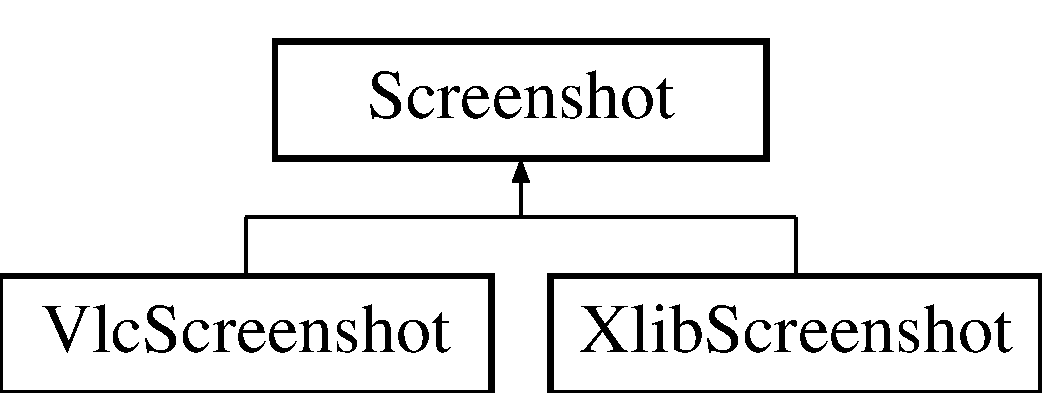
\includegraphics[height=2.000000cm]{classScreenshot}
\end{center}
\end{figure}
\subsection*{Public Member Functions}
\begin{DoxyCompactItemize}
\item 
virtual float \hyperlink{classScreenshot_a6f32c6952513af976d97f11871e679d3}{get\+Screen\+Crop} (Magick\+::\+Image \&result, const Magick\+::\+Geometry \&d)=0
\begin{DoxyCompactList}\small\item\em Provide a crop of the requested geometry. \end{DoxyCompactList}\item 
virtual void \hyperlink{classScreenshot_a2af036d2e54e9e96ac22a50d90ec17ec}{take\+Screenshot} ()\hypertarget{classScreenshot_a2af036d2e54e9e96ac22a50d90ec17ec}{}\label{classScreenshot_a2af036d2e54e9e96ac22a50d90ec17ec}

\begin{DoxyCompactList}\small\item\em Take a screenshot; this is for implementations where it is faster to only capture the screen once. \end{DoxyCompactList}\end{DoxyCompactItemize}


\subsection{Detailed Description}
Interface for capturing screen areas. 

\subsection{Member Function Documentation}
\index{Screenshot@{Screenshot}!get\+Screen\+Crop@{get\+Screen\+Crop}}
\index{get\+Screen\+Crop@{get\+Screen\+Crop}!Screenshot@{Screenshot}}
\subsubsection[{\texorpdfstring{get\+Screen\+Crop(\+Magick\+::\+Image \&result, const Magick\+::\+Geometry \&d)=0}{getScreenCrop(Magick::Image &result, const Magick::Geometry &d)=0}}]{\setlength{\rightskip}{0pt plus 5cm}virtual float Screenshot\+::get\+Screen\+Crop (
\begin{DoxyParamCaption}
\item[{Magick\+::\+Image \&}]{result, }
\item[{const Magick\+::\+Geometry \&}]{d}
\end{DoxyParamCaption}
)\hspace{0.3cm}{\ttfamily [pure virtual]}}\hypertarget{classScreenshot_a6f32c6952513af976d97f11871e679d3}{}\label{classScreenshot_a6f32c6952513af976d97f11871e679d3}


Provide a crop of the requested geometry. 


\begin{DoxyParams}[1]{Parameters}
\mbox{\tt out}  & {\em result} & the resulting image \\
\hline
 & {\em d} & the geometry saved in the result, relative to the complete screen \\
\hline
\end{DoxyParams}
\begin{DoxyReturn}{Returns}
the time in seconds required 
\end{DoxyReturn}


Implemented in \hyperlink{classXlibScreenshot_a6fc6b8262ef4d174804972fa5bb046be}{Xlib\+Screenshot}, and \hyperlink{classVlcScreenshot_a2edc869b862ef8569de2c680c7621d0b}{Vlc\+Screenshot}.



The documentation for this class was generated from the following file\+:\begin{DoxyCompactItemize}
\item 
screenshot.\+h\end{DoxyCompactItemize}

\hypertarget{classTripleScreenBorderProvider}{}\section{Triple\+Screen\+Border\+Provider Class Reference}
\label{classTripleScreenBorderProvider}\index{Triple\+Screen\+Border\+Provider@{Triple\+Screen\+Border\+Provider}}


An implementation of \hyperlink{classBorderProvider}{Border\+Provider}, accessing three monitors via the Screen\+Shot class.  




{\ttfamily \#include $<$triplescreenborderprovider.\+h$>$}

Inheritance diagram for Triple\+Screen\+Border\+Provider\+:\begin{figure}[H]
\begin{center}
\leavevmode
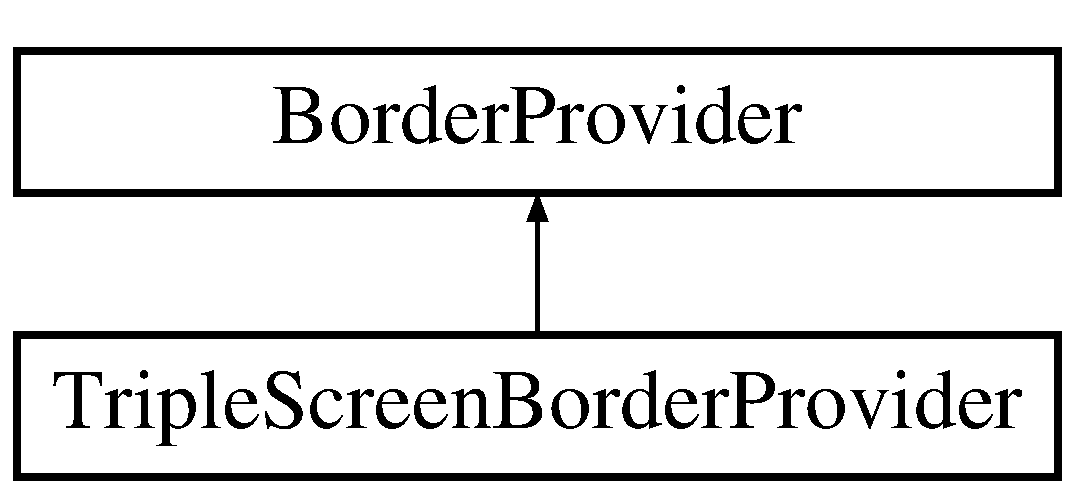
\includegraphics[height=2.000000cm]{classTripleScreenBorderProvider}
\end{center}
\end{figure}
\subsection*{Public Member Functions}
\begin{DoxyCompactItemize}
\item 
void \hyperlink{classTripleScreenBorderProvider_a045ee7528bf524af4b8fe48267a0cc9a}{retrieve\+Borders} (Magick\+::\+Image \&right, Magick\+::\+Image \&top, Magick\+::\+Image \&left, Magick\+::\+Image \&bottom) override\hypertarget{classTripleScreenBorderProvider_a045ee7528bf524af4b8fe48267a0cc9a}{}\label{classTripleScreenBorderProvider_a045ee7528bf524af4b8fe48267a0cc9a}

\begin{DoxyCompactList}\small\item\em This function creates a shot of each border; the rgb constructor can then use it to create the L\+ED data. \end{DoxyCompactList}\end{DoxyCompactItemize}


\subsection{Detailed Description}
An implementation of \hyperlink{classBorderProvider}{Border\+Provider}, accessing three monitors via the Screen\+Shot class. 

The documentation for this class was generated from the following files\+:\begin{DoxyCompactItemize}
\item 
triplescreenborderprovider.\+h\item 
triplescreenborderprovider.\+cpp\end{DoxyCompactItemize}

\hypertarget{classVlcScreenshot}{}\section{Vlc\+Screenshot Class Reference}
\label{classVlcScreenshot}\index{Vlc\+Screenshot@{Vlc\+Screenshot}}


An implementation of the \hyperlink{classScreenshot}{Screenshot} interface; it reads from a video stream provided by vlc. Not finished!  




{\ttfamily \#include $<$vlcscreenshot.\+h$>$}

Inheritance diagram for Vlc\+Screenshot\+:\begin{figure}[H]
\begin{center}
\leavevmode
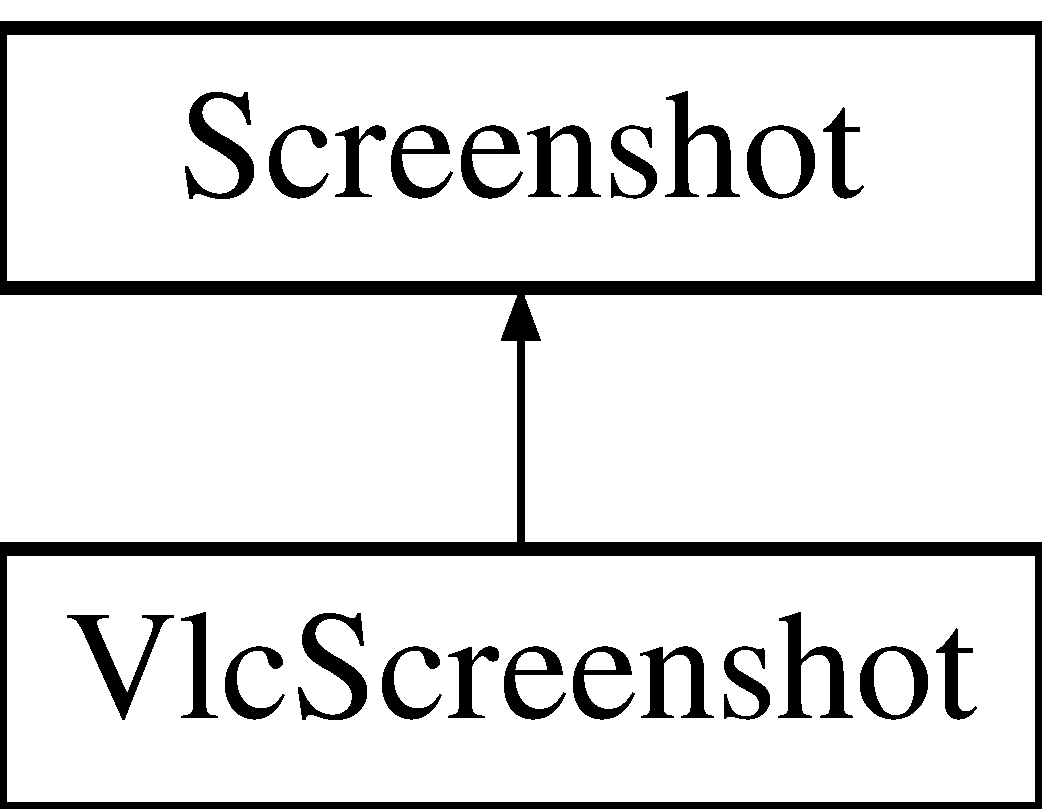
\includegraphics[height=2.000000cm]{classVlcScreenshot}
\end{center}
\end{figure}
\subsection*{Public Member Functions}
\begin{DoxyCompactItemize}
\item 
float \hyperlink{classVlcScreenshot_a2edc869b862ef8569de2c680c7621d0b}{get\+Screen\+Crop} (Magick\+::\+Image \&result, const Magick\+::\+Geometry \&d) override
\begin{DoxyCompactList}\small\item\em Crop the requested geometry from the last screenshot. \end{DoxyCompactList}\item 
void \hyperlink{classVlcScreenshot_a2d577851637459ce255eb4108ed8e0d8}{take\+Screenshot} () override\hypertarget{classVlcScreenshot_a2d577851637459ce255eb4108ed8e0d8}{}\label{classVlcScreenshot_a2d577851637459ce255eb4108ed8e0d8}

\begin{DoxyCompactList}\small\item\em Read the vlc stream. \end{DoxyCompactList}\end{DoxyCompactItemize}


\subsection{Detailed Description}
An implementation of the \hyperlink{classScreenshot}{Screenshot} interface; it reads from a video stream provided by vlc. Not finished! 

\subsection{Member Function Documentation}
\index{Vlc\+Screenshot@{Vlc\+Screenshot}!get\+Screen\+Crop@{get\+Screen\+Crop}}
\index{get\+Screen\+Crop@{get\+Screen\+Crop}!Vlc\+Screenshot@{Vlc\+Screenshot}}
\subsubsection[{\texorpdfstring{get\+Screen\+Crop(\+Magick\+::\+Image \&result, const Magick\+::\+Geometry \&d) override}{getScreenCrop(Magick::Image &result, const Magick::Geometry &d) override}}]{\setlength{\rightskip}{0pt plus 5cm}float Vlc\+Screenshot\+::get\+Screen\+Crop (
\begin{DoxyParamCaption}
\item[{Magick\+::\+Image \&}]{result, }
\item[{const Magick\+::\+Geometry \&}]{d}
\end{DoxyParamCaption}
)\hspace{0.3cm}{\ttfamily [override]}, {\ttfamily [virtual]}}\hypertarget{classVlcScreenshot_a2edc869b862ef8569de2c680c7621d0b}{}\label{classVlcScreenshot_a2edc869b862ef8569de2c680c7621d0b}


Crop the requested geometry from the last screenshot. 


\begin{DoxyParams}{Parameters}
{\em result} & the resulting image \\
\hline
{\em d} & the dimensions the image will be; these are the dimensions cropped from the screenshot \\
\hline
\end{DoxyParams}
\begin{DoxyReturn}{Returns}
the time in seconds required 
\end{DoxyReturn}


Implements \hyperlink{classScreenshot_a6f32c6952513af976d97f11871e679d3}{Screenshot}.



The documentation for this class was generated from the following files\+:\begin{DoxyCompactItemize}
\item 
vlcscreenshot.\+h\item 
vlcscreenshot.\+cpp\end{DoxyCompactItemize}

\hypertarget{classXlibScreenshot}{}\section{Xlib\+Screenshot Class Reference}
\label{classXlibScreenshot}\index{Xlib\+Screenshot@{Xlib\+Screenshot}}


An implementation of the \hyperlink{classScreenshot}{Screenshot} interface; uses xlib.  




{\ttfamily \#include $<$xlibscreenshot.\+h$>$}

Inheritance diagram for Xlib\+Screenshot\+:\begin{figure}[H]
\begin{center}
\leavevmode
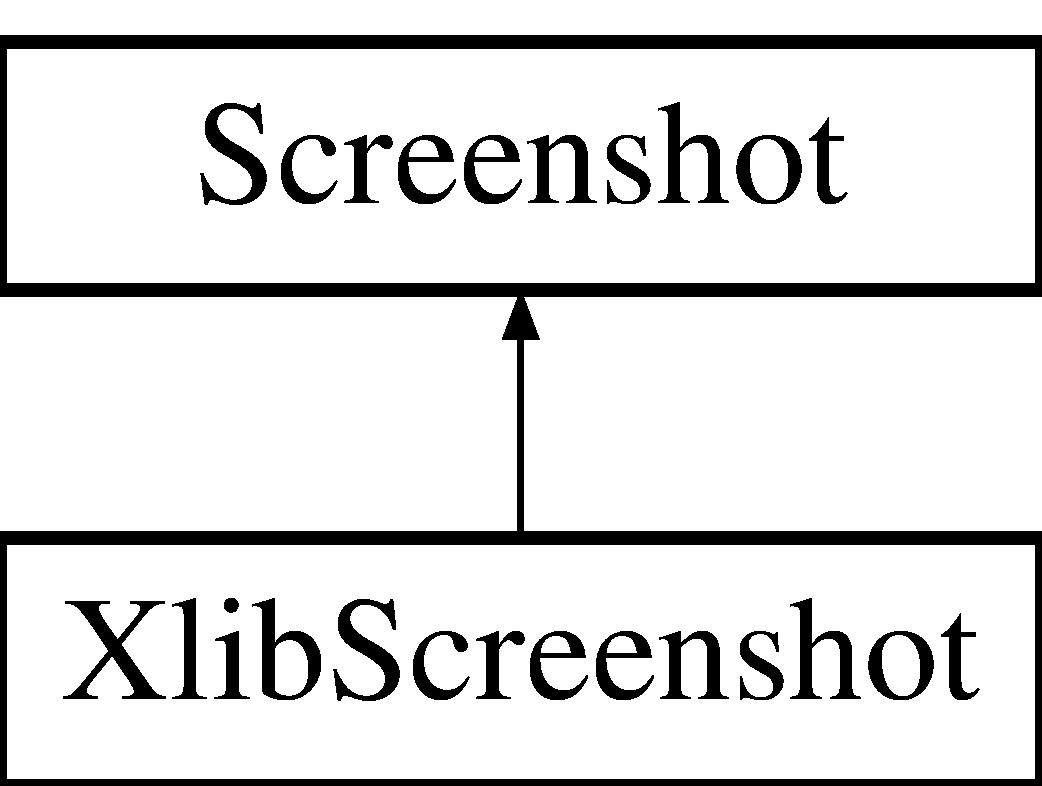
\includegraphics[height=2.000000cm]{classXlibScreenshot}
\end{center}
\end{figure}
\subsection*{Public Member Functions}
\begin{DoxyCompactItemize}
\item 
float \hyperlink{classXlibScreenshot_a6fc6b8262ef4d174804972fa5bb046be}{get\+Screen\+Crop} (Magick\+::\+Image \&result, const Magick\+::\+Geometry \&d) override
\begin{DoxyCompactList}\small\item\em take\+Screenshot Take a screenshot, converting it to a Magick++ image \end{DoxyCompactList}\end{DoxyCompactItemize}


\subsection{Detailed Description}
An implementation of the \hyperlink{classScreenshot}{Screenshot} interface; uses xlib. 

\subsection{Member Function Documentation}
\index{Xlib\+Screenshot@{Xlib\+Screenshot}!get\+Screen\+Crop@{get\+Screen\+Crop}}
\index{get\+Screen\+Crop@{get\+Screen\+Crop}!Xlib\+Screenshot@{Xlib\+Screenshot}}
\subsubsection[{\texorpdfstring{get\+Screen\+Crop(\+Magick\+::\+Image \&result, const Magick\+::\+Geometry \&d) override}{getScreenCrop(Magick::Image &result, const Magick::Geometry &d) override}}]{\setlength{\rightskip}{0pt plus 5cm}float Xlib\+Screenshot\+::get\+Screen\+Crop (
\begin{DoxyParamCaption}
\item[{Magick\+::\+Image \&}]{result, }
\item[{const Magick\+::\+Geometry \&}]{d}
\end{DoxyParamCaption}
)\hspace{0.3cm}{\ttfamily [override]}, {\ttfamily [virtual]}}\hypertarget{classXlibScreenshot_a6fc6b8262ef4d174804972fa5bb046be}{}\label{classXlibScreenshot_a6fc6b8262ef4d174804972fa5bb046be}


take\+Screenshot Take a screenshot, converting it to a Magick++ image 


\begin{DoxyParams}{Parameters}
{\em result} & the resulting image \\
\hline
{\em d} & the dimensions the image will be; these are the dimensions requested from X \\
\hline
\end{DoxyParams}
\begin{DoxyReturn}{Returns}
the time in seconds required 
\end{DoxyReturn}


Implements \hyperlink{classScreenshot_a6f32c6952513af976d97f11871e679d3}{Screenshot}.



The documentation for this class was generated from the following files\+:\begin{DoxyCompactItemize}
\item 
xlibscreenshot.\+h\item 
xlibscreenshot.\+cpp\end{DoxyCompactItemize}

%--- End generated contents ---

% Index
\backmatter
\newpage
\phantomsection
\clearemptydoublepage
\addcontentsline{toc}{chapter}{Index}
\printindex

\end{document}
